%%%%%%%%%%%%%%%%%%%%%%%%%%%%%%%%%%%%%%%%%%%%%%%%%%%%%%%%%%%%%%%%%%%%%
   \section{Design}
%%%%%%%%%%%%%%%%%%%%%%%%%%%%%%%%%%%%%%%%%%%%%%%%%%%%%%%%%%%%%%%%%%%%%




\begin{frame}{Component diagram}
	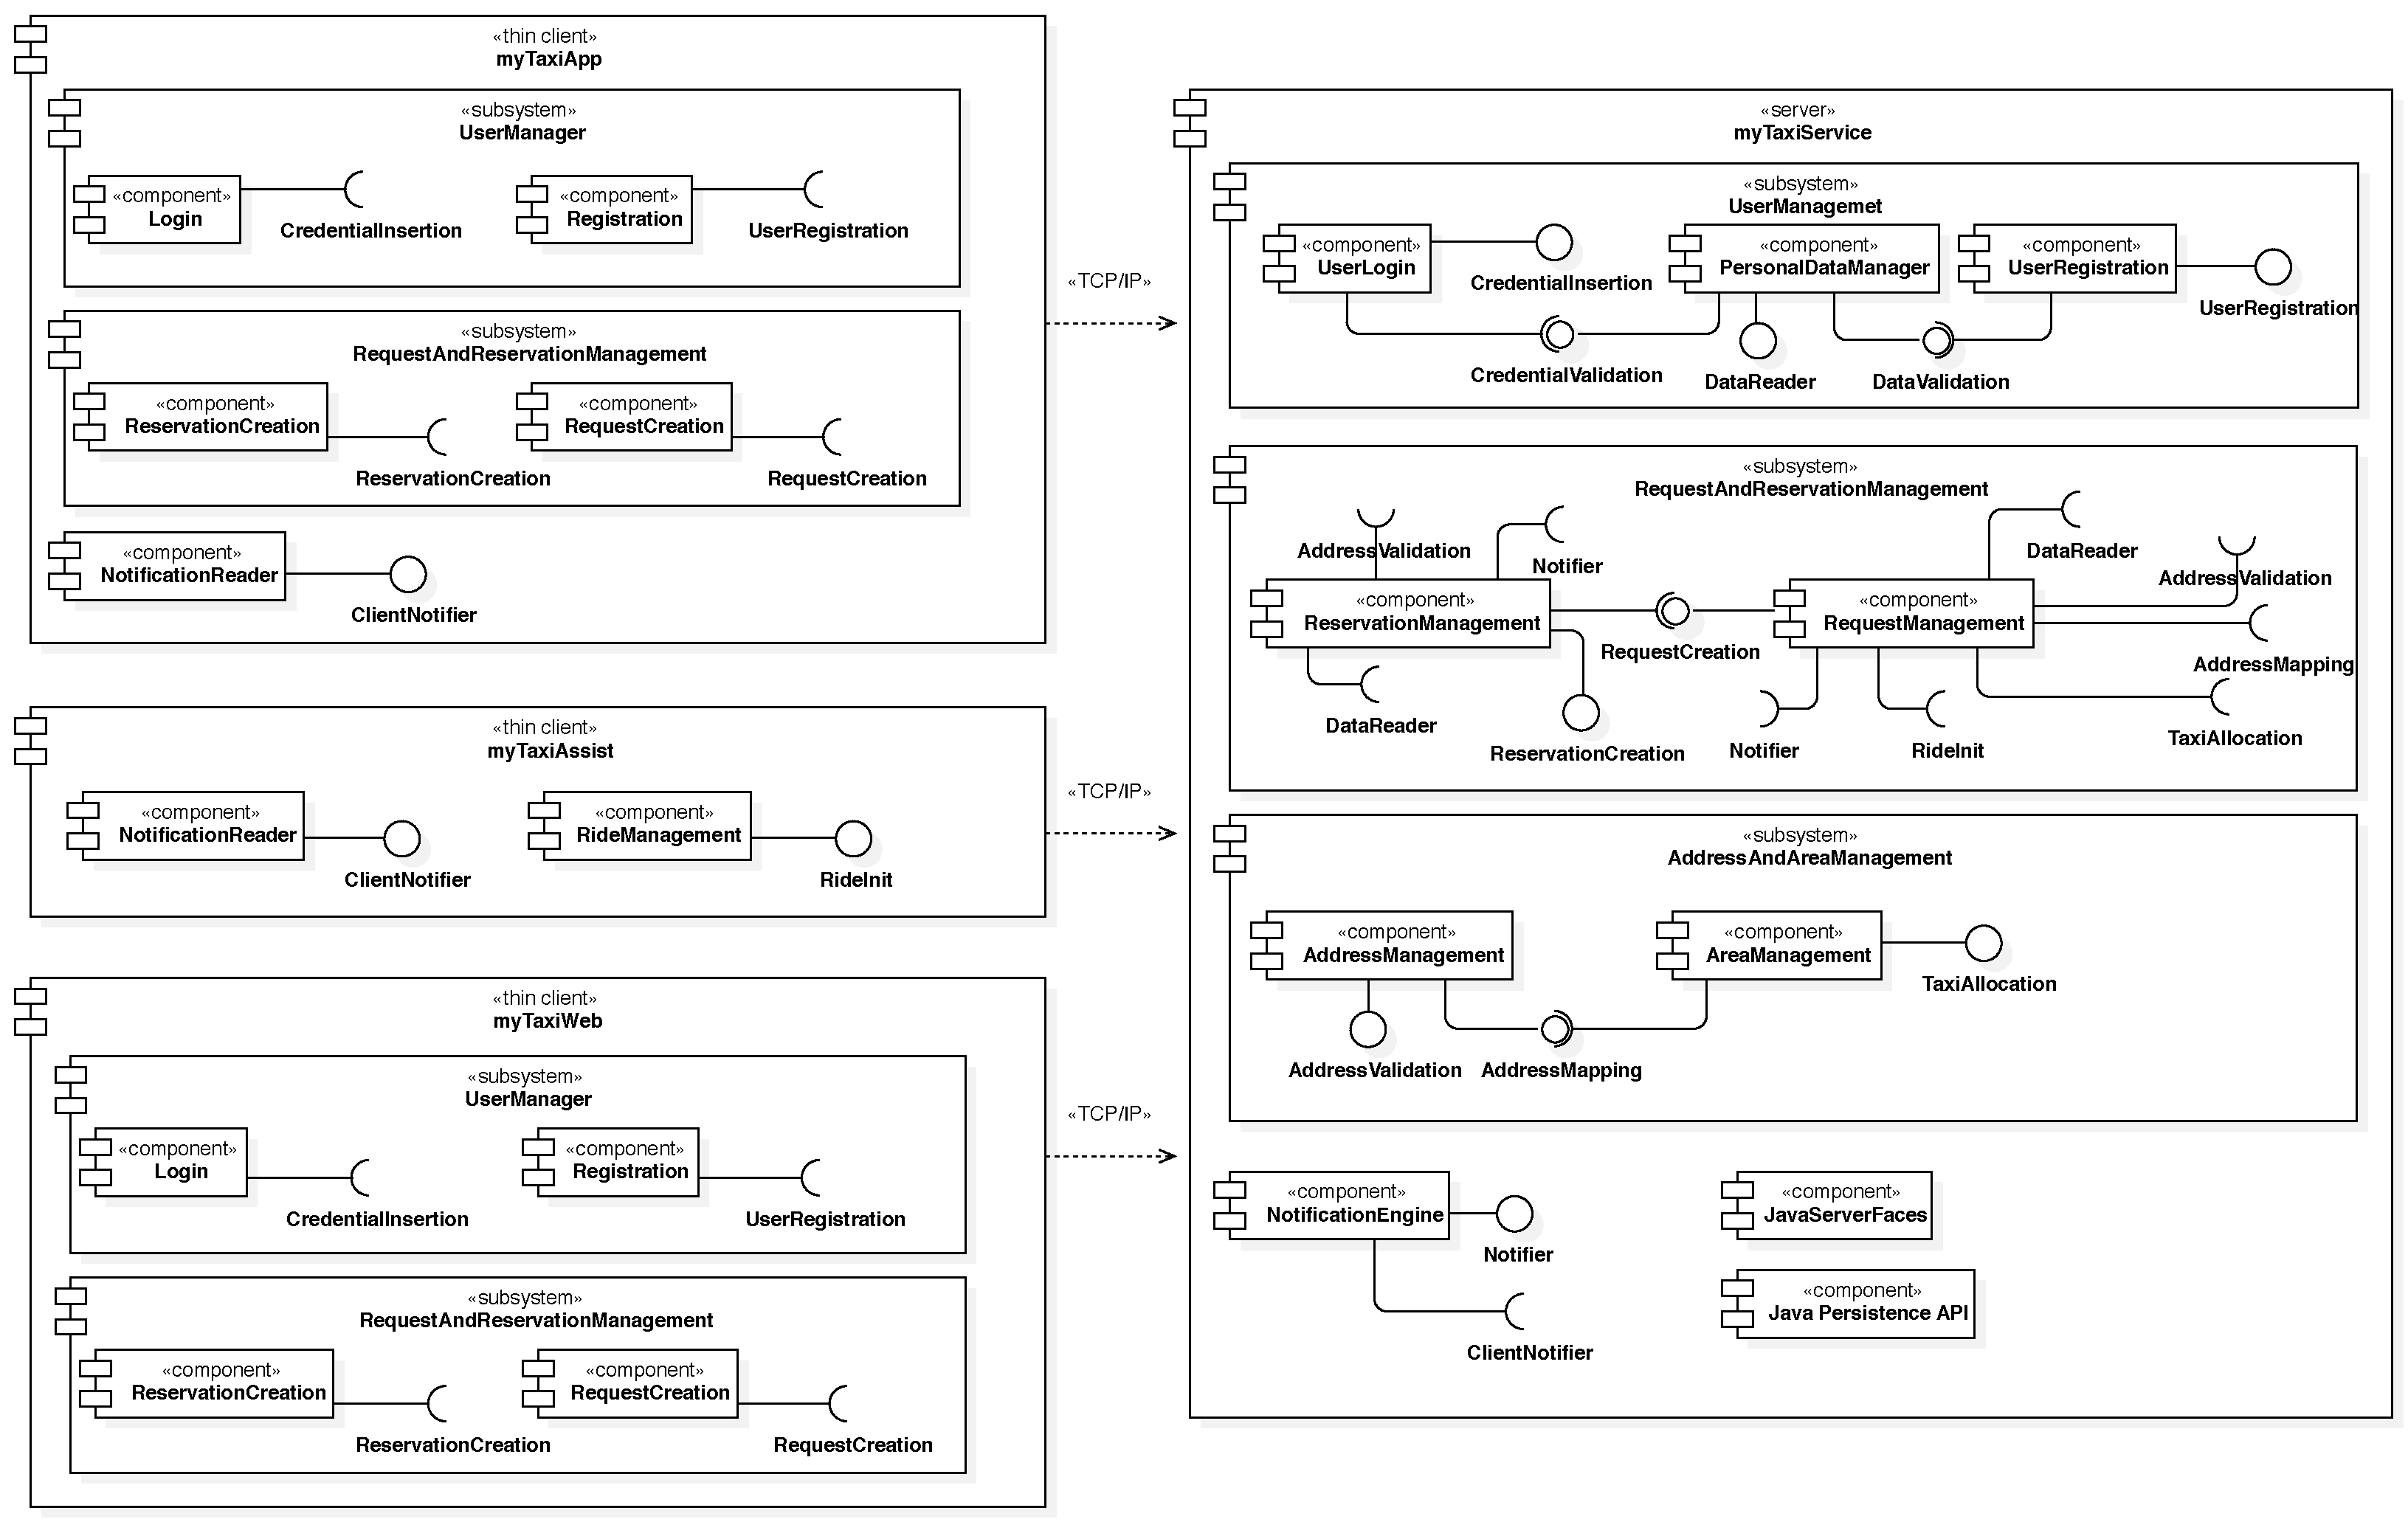
\includegraphics[width=\textwidth ]{img/ComponentView__ComponentDiagram_1}
\end{frame}





\begin{frame}[allowframebreaks]{Component interfaces}
	
\newcommand{\cW}{3.4cm}
\newcommand{\iW}{3.4cm}

\scriptsize

\begin{tabularx}{\textwidth}{ >{\ttfamily\bfseries}C{\cW} >{\ttfamily}C{\iW} >{\tiny}X }\toprule%
%
\normalfont\textbf{Component} & \normalfont\textbf{Interfaces} & \normalfont\scriptsize\textbf{Description}
\\%
\toprule%
%
	\multirow{4}{*}{AddressManagement}%
	&% 
	AddressMapping%
	&%
	\parbox{\cellwidth}{Provides the methods to map addresses into the system, returning the corresponding area.}%
%	
	\\\cmidrule(lr){2-3}%
%
	&%
	AddressValidation% 
	&%
	\parbox{\cellwidth}{Offers the methods to validate addresses, checking their existence in the database. Also converts addresses in GPS coordinates and vice versa.	}%
%	
\\\midrule%
%
	AreaManagement% 
	&% 
	TaxiAllocation% 
	&% 
	\parbox{\cellwidth}{Provides the methods for managing the taxi allocation (e.g., enqueue and dequeue, and the change of a taxi availability).}%
	\\% 
\midrule%
%
	RequestManagement% 
	&% 
	RequestCreation% 
	&% 
	\parbox{\cellwidth}{Offers the methods to make a request. It validates data, interacts with the required components to allocate a taxi and stores the request in the database.}%	
\\% 
\bottomrule%	
\end{tabularx}%

%%	
%\\% 
%\midrule%
%%
%	NotificationEngine% 
%	&% 
%	Notifier% 
%	&% 
%	Provides the methods for the notification of client systems.%
%%	
%\\\midrule%
%%
%	NotificationReader% 
%	&% 
%	ClientNotifier% 
%	&% 
%	Provides the methods to notify the customers.%
%%	
%\\\midrule%
%%


\begin{tabularx}{\textwidth}{ >{\ttfamily\bfseries}C{\cW} >{\ttfamily}C{\iW} >{\tiny}X }\toprule%
%
\normalfont\textbf{Component} & \normalfont\textbf{Interfaces} & \normalfont\scriptsize\textbf{Description}
\\\toprule%
%
	\multirow{7}{*}{PersonalDataManager}%
	&% 
	CredentialValidation% 
	&% 
	\parbox{\cellwidth}{Provides the methods that check the personal credentials in the database.}%
%	
	\\\cmidrule(lr){2-3}%
%	
	&%
	DataValidation%
	&%
	\parbox{\cellwidth}{Provides all the methods to validate personal data, for instance the correctness of the name (it cannot contain numbers) or of a birthdate (it shall not be in the future).}%
%	
	\\\cmidrule(lr){2-3}%
%	
	&%
	DataReader%
	&%
	\parbox{\cellwidth}{Offers the methods to access customer data, stored in the database.}%
%
\\\midrule%
%
	ReservationManagement% 
	&% 
	ReservationCreation% 
	&% 
	\parbox{\cellwidth}{Provides the methods to make a reservation. It interacts with other components for data validation and storing.}%
%%
%\\% 
%\midrule%
%%
%	RideManagement% 
%	&% 
%	RideInit% 
%	&% 
%	Provides the methods necessary to instantiate a ride for the driver. This component interacts also with the on board navigator.%
%%
%\\% 
%\midrule%
%%
%	UserLogin% 
%	&% 
%	CredentialInsertion% 
%	&% 
%	Offers the methods useful to log in a User (both a registered customer and a taxi driver). It interacts with \texttt{Per\-son\-al\-Data\-Man\-ager} component to complete the login and start the user session.%
%%	
%\\% 
%\midrule%
%%	
%	UserRegistration% 
%	&% 
%	UserRegistration% 
%	&% 
%	Provides the methods for the insertion of a new customer in the database, validating his data.%
%%	
\\% 
\bottomrule%	
\end{tabularx}%

	
	
	



\end{frame}




